\documentclass{article}
\usepackage[utf8]{inputenc}

\title{Homework No.2}
\author{Osamu Katagiri-Tanaka : A01212611}
\date{\today}

% import math symbols
\usepackage{amsmath, esint}
\usepackage{cancel}

% import continuous lists
\usepackage{enumitem}

% format margins and paper size
\usepackage{geometry}
\geometry{
	paper         = a4paper, % Change to letterpaper for US letter
	inner         = 2.5cm,   % Inner margin
	outer         = 2.5cm,   % Outer margin
	bindingoffset = 0.5cm,   % Binding offset
	top           = 1.5cm,   % Top margin
	bottom        = 1.5cm    % Bottom margin
}

% import figure handler
\usepackage{graphicx}

% import references handler
\usepackage[
    style     = ieee,         % references format style
    backend   = biber,        % choose the processing program
    natbib    = true,         % enable additional reference formats
    citestyle = numeric-comp, % enable multiple citations
    sortcites = true,         % sort references in multiple citations
    sorting   = nyt           % sort the reference table
]{biblatex}
\addbibresource{references.bib}

% Note that ‘d’ in the differential is conventionally set in roman.
\newcommand{\ud}{\,\mathrm{d}}

% Paragraph spacing
\setlength{\parskip}{0.2cm}           % spacing between paragraphs
\renewcommand{\baselinestretch}{1.25} % spacing between lines

\begin{document}

\maketitle

\section*{\emph{What will I achieve?}}
With this homework you will practice the use of the concepts and knowledge acquired throughout the corresponding topics.

\section*{Instructions}

\begin{enumerate}
\item \textit{Read \textbf{problem statement}, and collect the information that may be needed.}
\end{enumerate}

if the system initially is at $25^\circ C$

\begin{enumerate}[resume]
\item \textit{Make a \textbf{Sketch} (Diagram, process flow chart), indicating mass, linear or angular momentum (i.e. forces and torques) and energy interaction, and label each stream and boundaries as well.}
\end{enumerate}

See Figure \ref{fig_SKETCH}

\begin{figure}[h!]
\centering
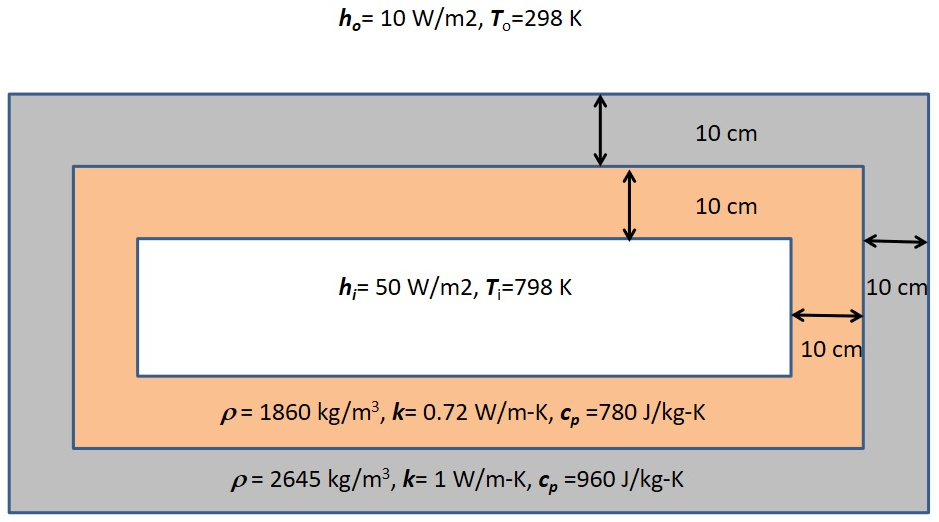
\includegraphics[width=0.75\textwidth]{./img/SKETCH.png}
\caption{Properties of a chimney}
\label{fig_SKETCH}
\end{figure}

\begin{enumerate}[resume]
\item \textit{List \textbf{Assumptions and Approximations} (sometimes they may be inferred by the sketch, but make them explicit) supported by equations if possible (geometric relationships, or fundamental equations).}
\end{enumerate}

\begin{enumerate}[resume]
\item \textit{\textbf{Physical Laws} (Fundamental Laws) must be written in full form, and terms can be dropped by the right selection of frame of reference, operating conditions, assumptions, simplifications or constraints.}
\end{enumerate}

\begin{enumerate}[resume]
\item \textit{\textbf{Physical constants} should be obtained from a reliable source (knowing this information by heart is always helpful ), geometric relations and formulae must be included as part of your analysis.}
\end{enumerate}

\begin{enumerate}[resume]
\item \textit{\textbf{Physical transport or thermodynamic properties} (Thermodynamic relations) should be evaluated, approximated, calculated or obtained from a reliable source.}
\end{enumerate}

\begin{enumerate}[resume]
\item \textit{\textbf{Calculations} are done including units. Any algebraic manipulation is recommended in few cases, because limits the step 8, but if needed should be done before using numerical values of constants, properties or variables.}
\end{enumerate}

\begin{enumerate}[resume]
\item \textit{\textbf{Reasoning} (Sensitivity analysis, what if), Verification (context), and Discussion should always be part of your answer to any problem, regardless the task requested.}
\end{enumerate}

\printbibliography[title={References}]
\end{document}